The \texttt{\pkglnk{view}} package manages general aspects of the application.
Among these are building the UI, managing the interaction between the \texttt{\pkglnk{model}} and the \texttt{\pkglnk{view}} and serialization.

The \texttt{\lnk{URLSerializer}} class manages the serialization of the applications state. 
Hence it needs the objects that are serialized and the recipients of the serialization.
The recipients must implement the \texttt{\lnk{SerializationObserver}} interface in order to update the serialization.
Note that the \texttt{\lnk{URLSerializer}} needs a polling delay time in milliseconds for concurrency.

The \texttt{\lnk{App}} class builds the UI components and the associated actions. 
It also stores an instance of the \texttt{\hyperref[type:edu.kit.wavelength.client.view.execution.Executor]} class.
Note that the \texttt{\lnk{App}} class works as a singleton, guaranteeing that only one instance exists and is accessed using a static method.
Hence each \texttt{\hyperref[type:edu.kit.wavelength.client.view.action.Action]{Action}} can access the \texttt{\lnk{App}}
in order to use the \texttt{\pkglnk{model}} via the \texttt{\hyperref[type:edu.kit.wavelength.client.view.execution.Executor]{Executor}} class
or get UI components by calling the respective methods.

\begin{figure}[H]
	\centering
	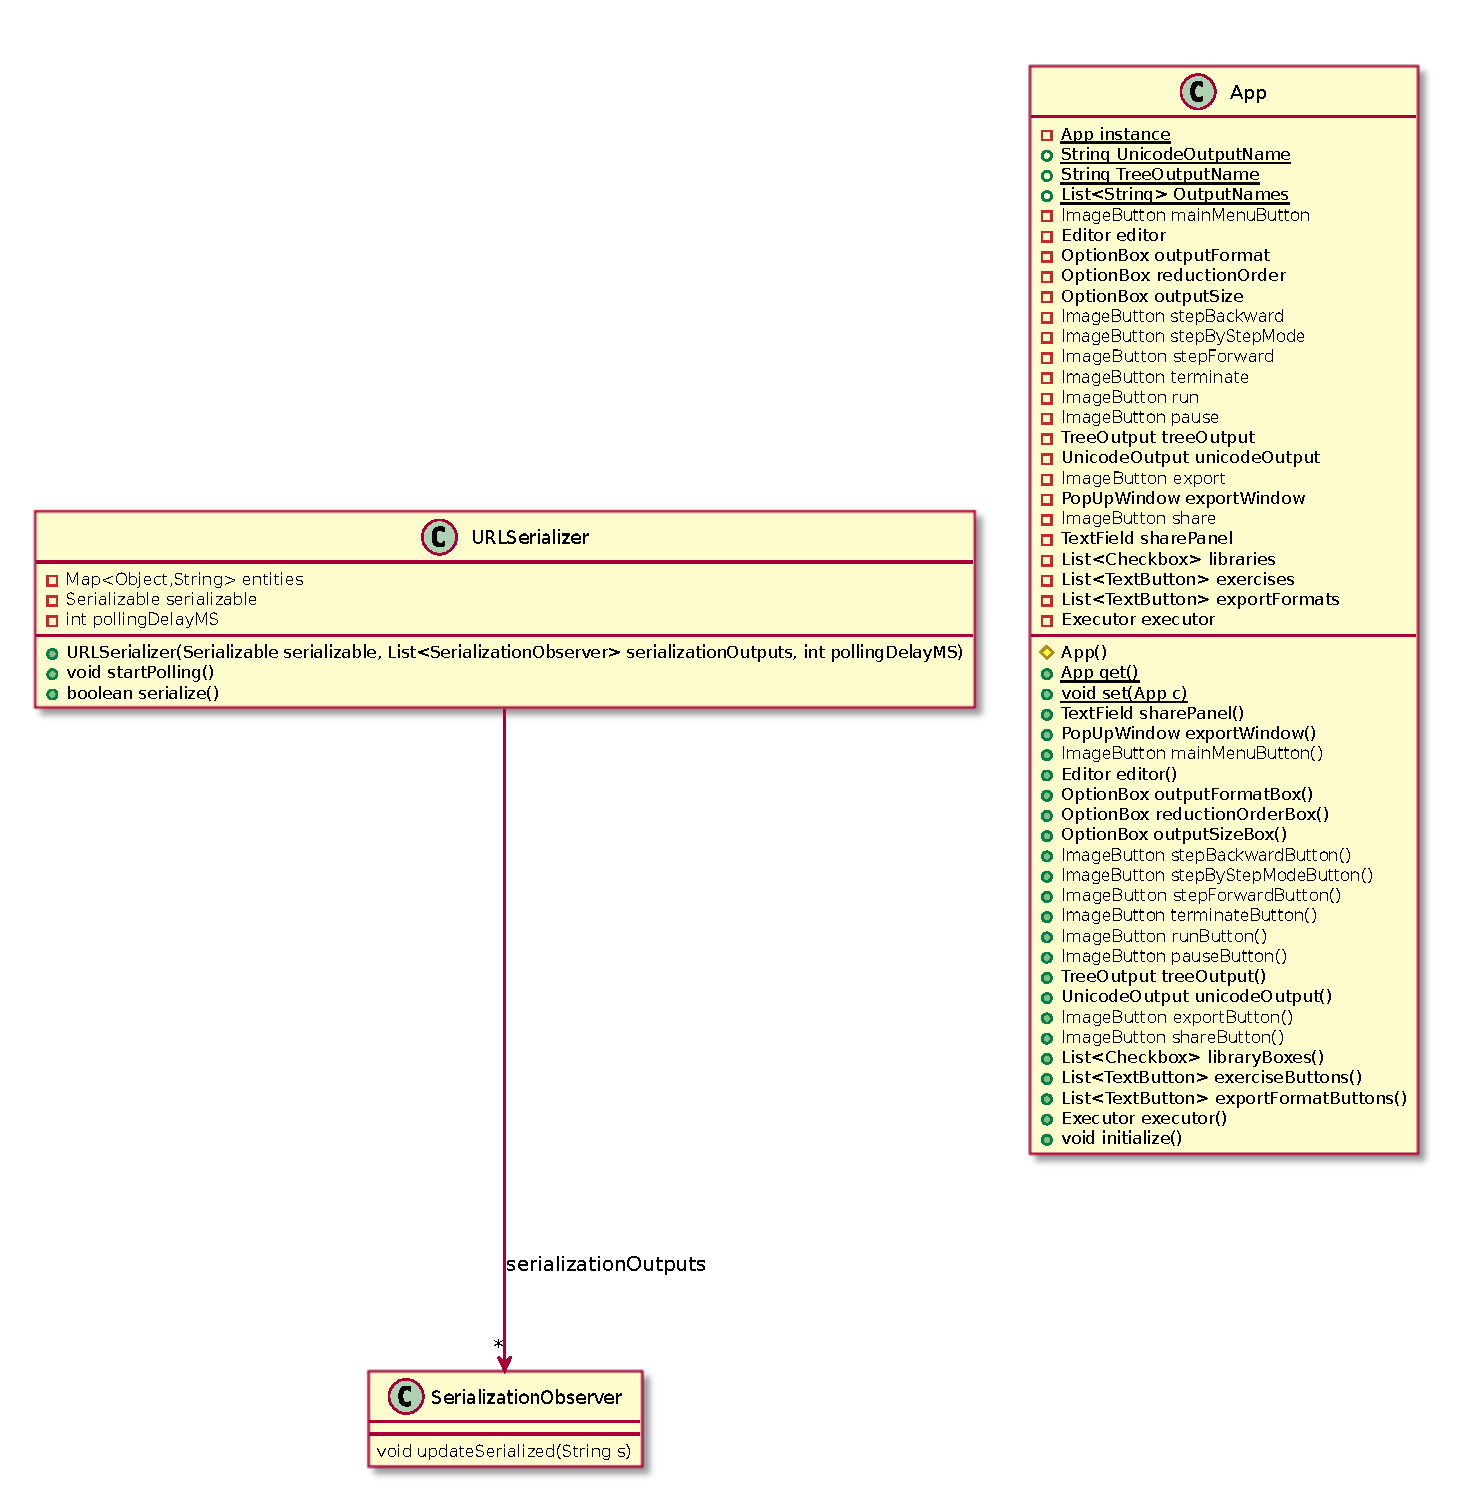
\includegraphics[width=0.7\textwidth]{packageDiagrams/viewPackage}
\end{figure}
